
% ################################# Paragraph #################################
% AB3 Structures and Training
- XYZ unique AB3 Structures, 259 unique prototypes.  Substitute Ir and O, expand to minimum Ir-O distance > XYZ
- followed same procedure as in 3.1, Training Set of 35 structures, 8 of which are \ce{IrO_3}
- Describe initial training and training after first 10 DFT structures

% ################################# Paragraph #################################
% P2 Analysis of \ce{IrO_3} Structures
% COMBAK Change alpha to actual greek symbol
- Describe convex hull, classes of structures (\ce{$\alpha$-AlF3} like, rutile like, and layered, should be segregated in hull plot)
- briefly describe structures within each class, cite in literature where appropriate

  % | - Figure | IrO3 Convergence Plot
\begin{figure}
\centering
\makebox[\textwidth][c]{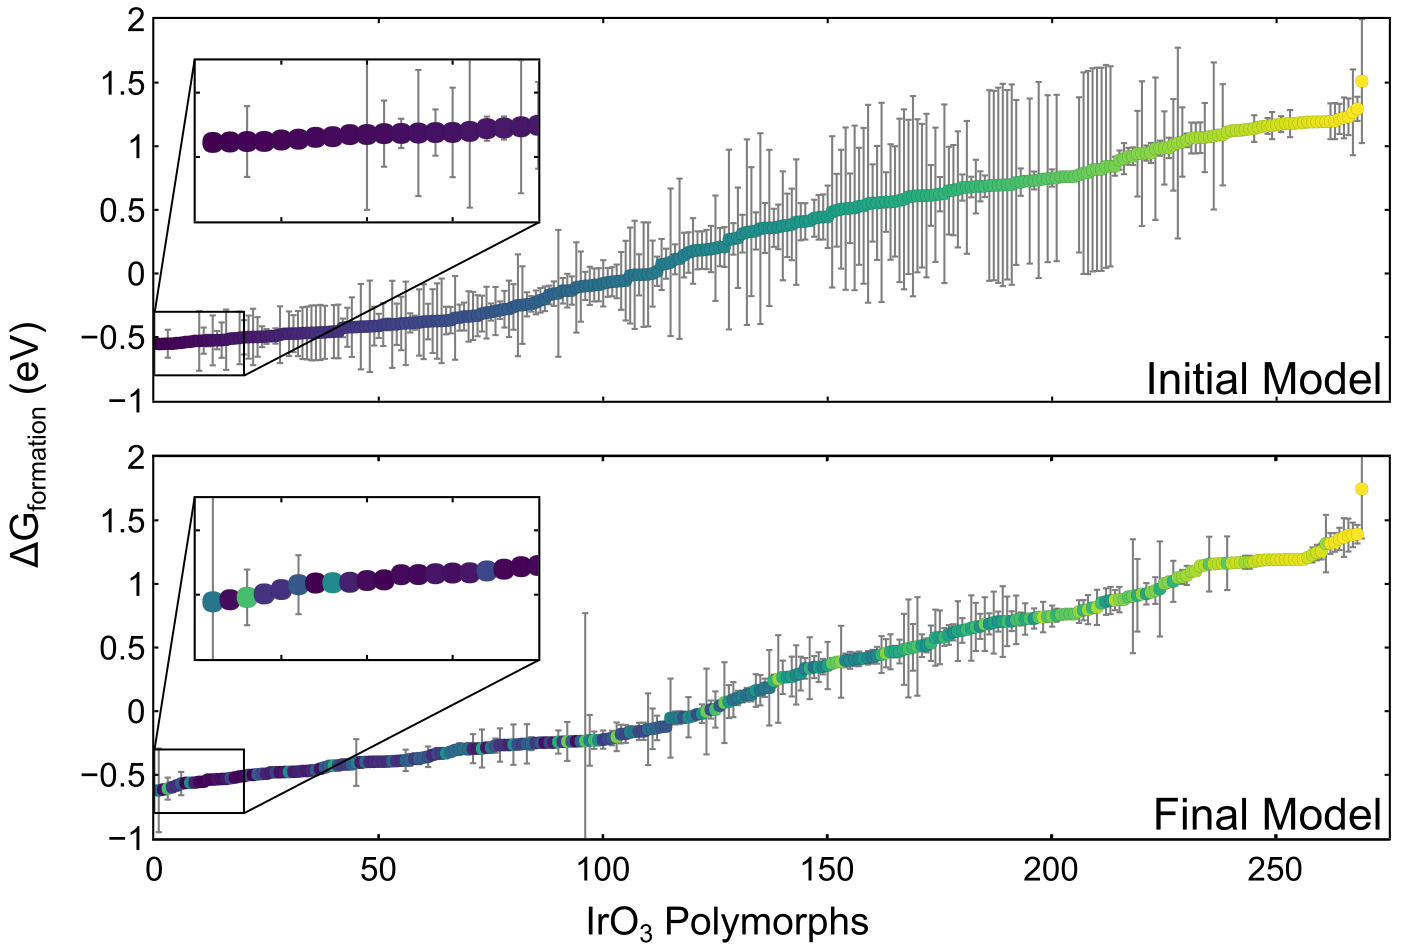
\includegraphics
  {02_figures/ml_convergence_plots/00_master__iro3-ml-conv_v6__200dpi__0__outplot.png}
  % {02_figures/ml_convergence_plots/iro3_ml_conv.png}
  }

\caption{\label{fig:convergence_plot_iro3_0}
  TEMP.
  }
\end{figure}
  % __|
